\section{Branchement des différents éléments}
	\subsection{Général}
	Afin de faire fonctionner le système, tous les éléments sur le schéma \ref{fig.general} doivent être branchés. Il faut suivre l’ordre suivant afin que tout fonctionne correctement:
	%
	\begin{enumerate}
		\item Alimenter le routeur fourni et attendre qu’il soit démarré
		\item Brancher deux câbles ethernet sur des ports libres (gris) du routeur
		\item Brancher un câble ethernet dans le raspberry pi et l’autre dans le pont
		\item Alimenter le raspberry pi et le pont, attendre un moment qu’ils démarrent
		\item Alimenter les deux terminaux, ils se connecteront au réseau automatiquement
	\end{enumerate}

Note : La base de données sur le raspberry pi démarre automatiquement, mais pas l’application \og serveur \fg{}, il faudra suivre la méthode suivante:
	%
	\begin{enumerate}
		\item Connecter en SSH avec \code{pi:raspberry}
		\item Naviguer vers 	\code{~/ByPass/server}
		\item Exécuter la commande \code{pm2 start server.js}
	\end{enumerate}
	
	\subsection{Pont}
	Le branchement du pont est relativement simple. Le LPC est connecté au port RJ45 afin de communiquer avec le serveur. Il est aussi connecté au module Xbee Contrôleur afin de recevoir les requêtes des terminaux et transmettre les réponses du serveur.
	
	\begin{figure}[h]
		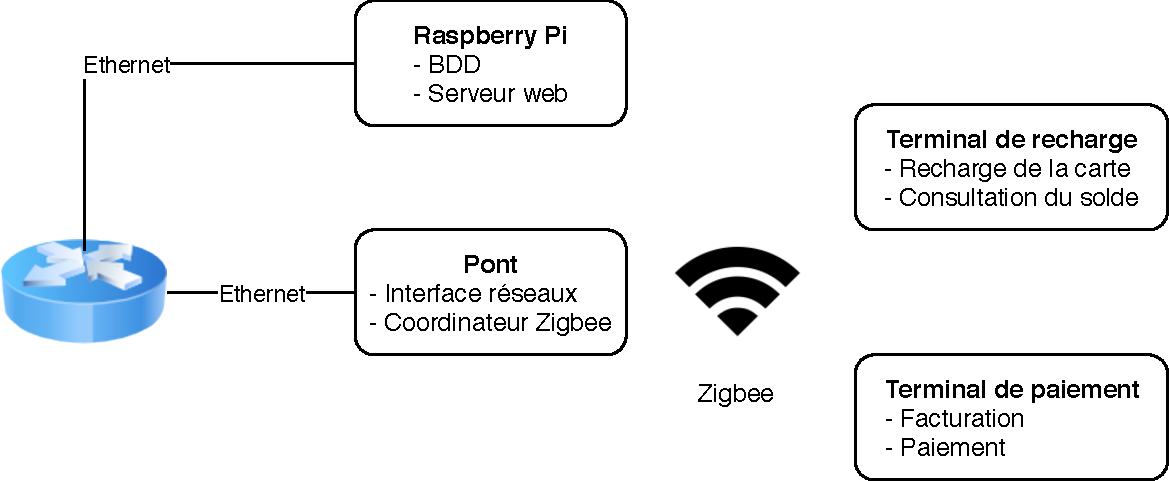
\includegraphics[width=\textwidth]{Pictures/Branchements/general}
		\caption{Schéma-bloc des composantes générales du prototype}
		\label{fig.general}
	\end{figure}
	
	\clearpage

	\begin{figure}[t]
		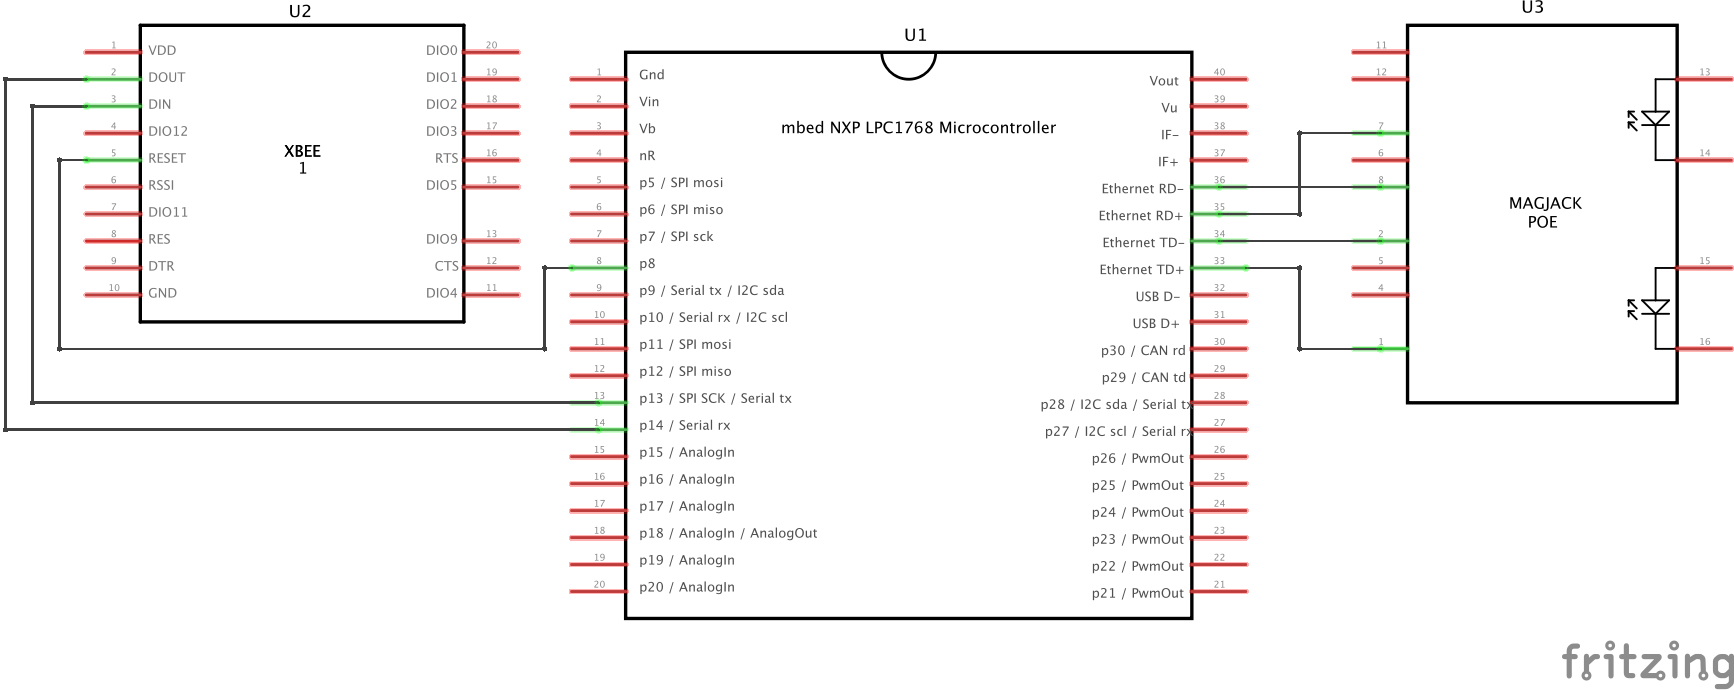
\includegraphics[width=\textwidth]{Pictures/Branchements/Pont}
		\caption{Schéma des branchements du pont}
		\label{fig.branchPont}
	\end{figure}

	\subsection{Terminal de paiement}
	L’alimentation se fait à grâce à une batterie Li-ion sa tension nominal étant beaucoup trop élevée par rapport à notre circuit nous utilisons un régulateur de tension à découpage de type buck (MP1564) pour abaisser la tension à 5VDC, ce type de régulateur a un excellent rendement ce qui est une caractéristique recherchée dans un application embarquée, le XBee et le détecteur RFID MFRC522 n’acceptent cependant pas le 5VDC, nous utilisons donc le régulateur de tensions 3.3V du LCP1768  pour son alimentation. 

	Le LCD est alimenté en 5VDC et est commandé par un interface de 4 bits en parallèles pour les données et de 2 pins pour l’activation du module et une pour lui indiquer s’il s’agit d’une commande ou d’un caractère. 

	Le détecteur RFID est interfacé en SPI (mosi, miso, sck et le ss) de plus une pin (IRQ) nous indique quand une carte est détectée et une pin pour le reset. Une fois la carte détectée le module nous retourne son identifiant via SPI.

	Finalement le XBee est interfacé en UART et possède une pin de plus pour le reset.

	\begin{figure}[p]
		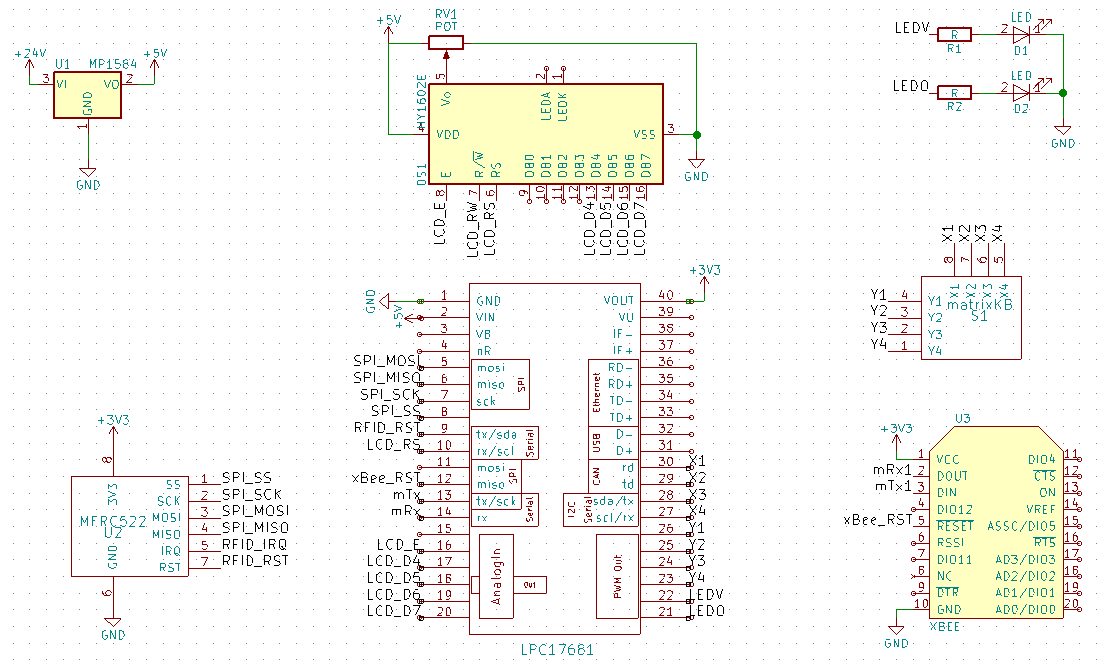
\includegraphics[width=\textwidth]{Pictures/Branchements/Terminal_Paiement}
		\caption{Schéma des branchements du terminal de paiement}
		\label{fig.branchPaiement}
	\end{figure}

	\begin{figure}[p]
		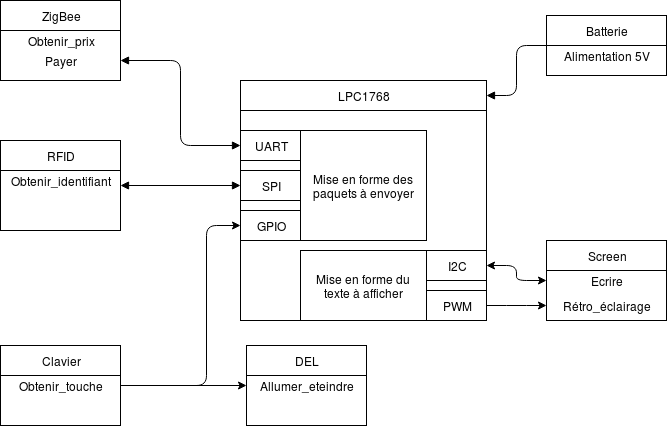
\includegraphics[width=\textwidth]{Pictures/Branchements/Paiement_Bloc}
		\caption{Schéma-bloc du terminal de paiement}
		\label{fig.blocPaiement}
	\end{figure}
		
	\subsection{Terminal de recharge}
	Tout comme le terminal de paiement l’alimentation se fait grâce à une batterie Li-ion. Sur ce montage, nous avons ajouté un régulateur de tension 12~V pour l’alimentation du monnayeur, étant donné que nous n’avions à notre disposition qu’un régulateur de tension linéaire de type~LM317. L'inconvénient avec ce type de régulateur est que beaucoup de puissance est dissipée dans ce dernier; c’est pour cela que nous avons rajouté le transistor MOSFET 2N7000 pour alimenter ou non le monnayeur. En appliquant une tension sur la \emph{gate} du 2N7000, nous connectons l’alimentation négative du monnayeur au GND, et ceci nous permet d'économiser beaucoup d’énergie. Le monnayeur quant à lui est un module qui se configure à l’aide d’une interface utilisateur sommaire, une fois configuré et lorsqu’une pièce est détectée, le monnayeur nous délivre $N$ flancs descendants ($N$ correspondant à la valeur de la pièce que nous avons configurée).

	\begin{figure}[p]
		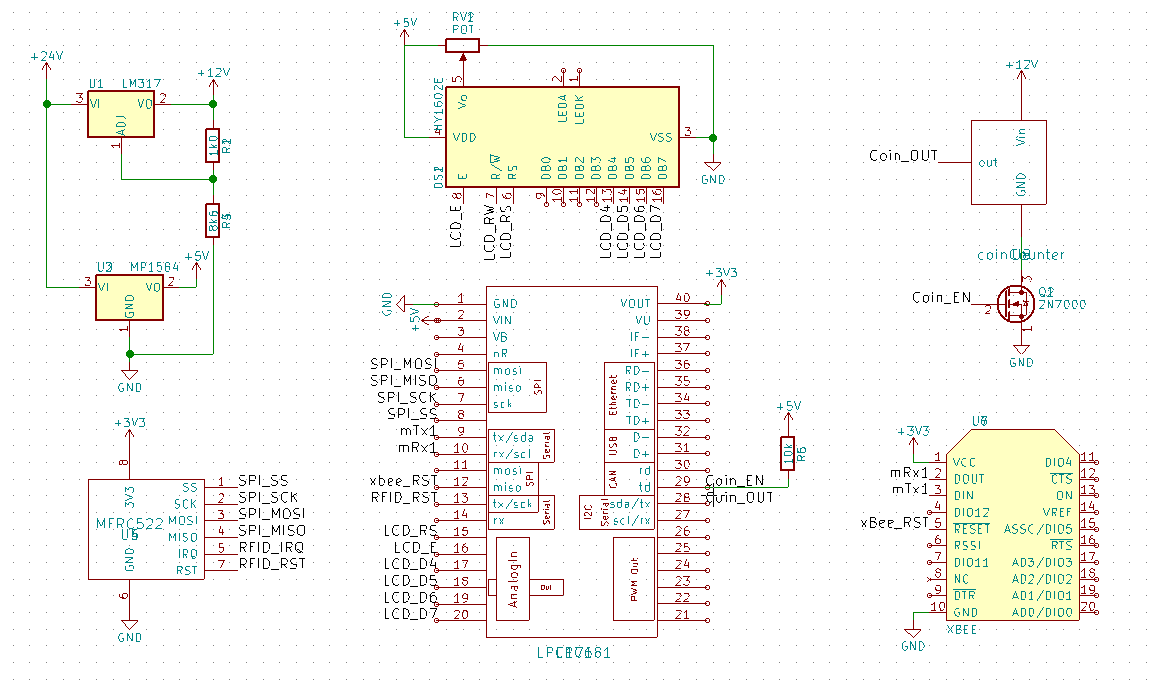
\includegraphics[width=\textwidth]{Pictures/Branchements/Terminal_Recharge}
		\caption{Schéma des branchements du terminal de recharge}
		\label{fig.branchRecharge}
	\end{figure}

	\begin{figure}[p]
		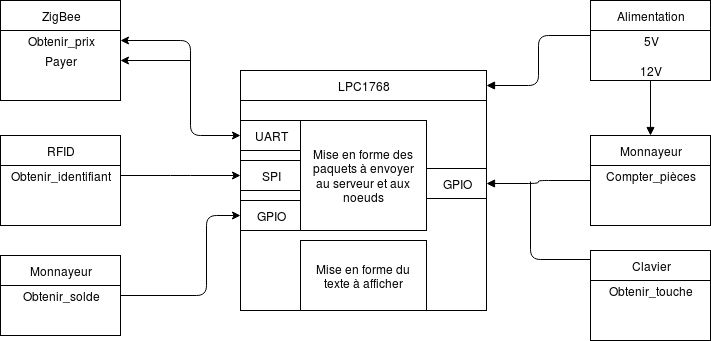
\includegraphics[width=\textwidth]{Pictures/Branchements/Recharge_Bloc}
		\caption{Schéma-bloc du terminal de recharge}
		\label{fig.blocRecharge}
	\end{figure}

	
	